\section{Problem 2-3 Degree distributions}

Select two networks, a small network with $N \le 250$ nodes from the Koblenz Network Collection KONECT and a larger network with $N \ge 2500$ nodes from the Stanford Large Network Dataset Collection SNAP. For each of the networks, provide the following plots. 

\begin{enumerate}
 \item Show the cumulative degree distribution of each network in a separate plot. Specifically, plot the degree $k_x \in \{1,...,N\}$ on the $x$-axis. 
 
 On the $y$-axis, plot $P(k \ge k_x)$ that denotes the probability of a randomly chosen node in the network having a degree of $k_x$ or higher. 
 
 Select appropriate scales for your plots!
 
 \item To each plot, add the cumulative degree distribution of a random graph with a corresponding number of nodes and edges (approximately!). 
 
 You are free to chose between the $G(N,L)$ and the $G(N,p)$ model for random graphs. 
 
 Average the degree counts over at least 10 samples from the random graph model. 
 
\end{enumerate}

Include your plots and a brief discussion of your findings in the PDF with your solution to this assignment. Also hand in your source code along with specific instructions on how to compile and run your program in a separate archive file.

\begin{figure}[h]
	\centering
	\begin{subfigure}{.5\textwidth}
		\centering
		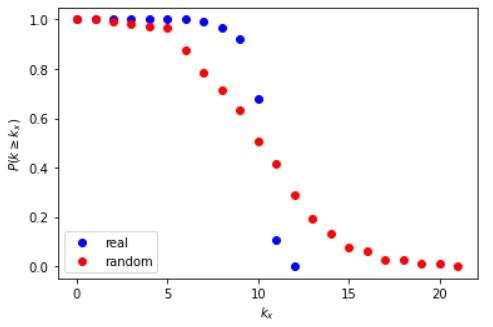
\includegraphics[width=\linewidth]{images/american_football.png}
		\caption{KONECT American Football network}
	\end{subfigure}%
	\begin{subfigure}{.5\textwidth}
		\centering
		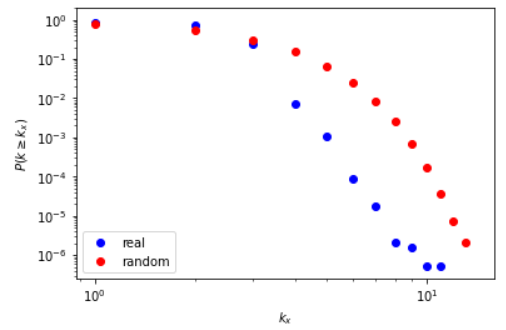
\includegraphics[width=\linewidth]{images/california_roads.png}
		\caption{SNAP roadNet-CA (log log scale)}
	\end{subfigure}
	\caption{Complementary cumulative distribution functions of the degree distributions}
	\label{fig:test}
\end{figure}

When averaging the degree distribution for both randomly created networks over 10 instances and comparing their complementary cumulative distribution functions (CCDF) to those of the real networks, one can identify interesting results. In both cases the probability for high degree nodes is overestimated by the random networks. This can be explained by the hard organisatorial and physical thresholds that the real networks impose. In case of the american football network, each team normally has the same amount of matches during a season except the case that additional relegation matches are scheduled. Also road networks normally have a physical threshold as not too many roads can intersect each other. The random networks and their underlying binomial distribution aim for softer boundaries in the degree distribution and therefore lead to overestimation. 

In case of the american football network, the random model even overestimates the amount of teams that have very few games in one season. As this is also rarely the case in reality and teams tend to have the same amount of matches, the CCDF of the real network remains on a plateau at the beginning while the CCDF of the random network already decreases in value. On the other hand, both real and random CCDF on the road networks seem to match at the beginning. 

This leads to the conclusion that both random networks cannot be identified as the generative model behind the real networks.